\documentclass[12pt]{article}
\usepackage[margin=1.0in]{geometry} %page layout
\usepackage[usenames,dvipsnames]{color} %color
\definecolor{light-gray}{gray}{0.95}
\definecolor{darkgreen}{rgb}{0,0.4,0}
\usepackage{graphicx, subfigure} %figures
\usepackage{url, hyperref} %cross-referencing
\usepackage{amsmath, amssymb} %math
\usepackage{listings} %source code
\lstset{breaklines=true,
breakindent=0pt,
prebreak=\mbox{\tiny$\searrow$},
postbreak=\mbox{{\color{blue}\tiny$\rightarrow$}},
numbers=left,
commentstyle=\color{darkgreen},
numberblanklines=false,
frame=single,
captionpos=b,
backgroundcolor=\color{light-gray}}
\usepackage[3D]{movie15} %for movies (needs hyperref)
	\newenvironment{changemargin}[2]
	{
	  	\begin{list}{}
		{
			\setlength{\topsep}{0pt}%
			\setlength{\leftmargin}{#1}%
			\setlength{\rightmargin}{#2}%
			\setlength{\listparindent}{\parindent}%
			\setlength{\itemindent}{\parindent}%
			\setlength{\parsep}{\parskip}%
		}
	  	\item[]
		}
		{\end{list}
	}
\author{Salman Aslam\\Georgia Tech}
\title{Tracking Results\\PCA}
\date{}
\begin{document}
\maketitle
\rule[0pt]{\textwidth}{1pt}
\tableofcontents
\rule[0pt]{\textwidth}{1pt}
%=========================
\section{Introduction}
%=========================
In this report, our goal is to present tracking error results for our PCA based tracker.

								\begin{figure}[t]
								\centering
								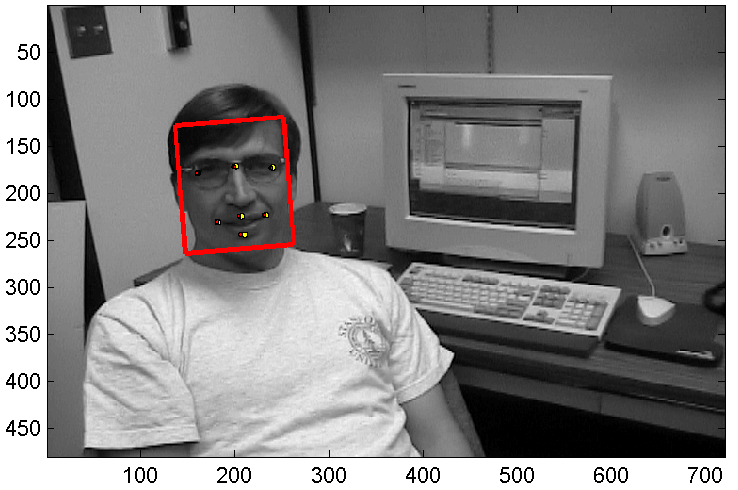
\includegraphics[width=0.7\textwidth]{temp/results_pca__trk_dudek_0007.png}
								\caption{Computing tracking error.  The larger yellow circles indicate ground truth feature points.  The smaller red circles indicate estimated feature points.  Tracking error is computed using the rms error between the ground truth feature points and the estimated feature points.  In this particular frame, the tracking error is 2.57.}
								\label{fig:results_pca__trk_dudek_0007}
								\end{figure}
%=========================
\section{Experiments}
%=========================
A PCA based tracker using our previously described 5-component tracker comprising appearance, representation, observation, motion and inference models was run on 6 publicly available datasets, Dudek, davidin300, sylv, fish, car4 and car11.  These datasets can be downloaded from~\cite{2008_JNL_subspaceTRK_Ross}.

Tracking error was measured on each of these datasets using the error between ground truth feature points and estimated feature points as shown in Figure~\ref{fig:results_pca__trk_dudek_0007} for the Dudek sequence.

									\begin{figure}[t]
									\centering
									\subfigure[Dudek.]{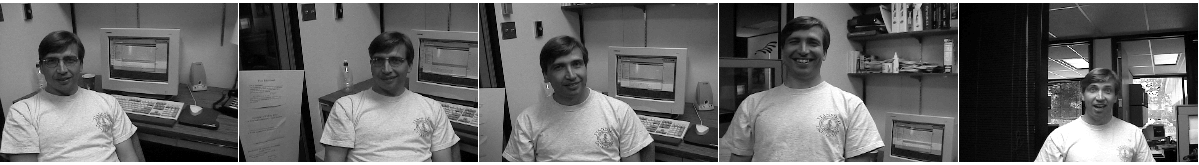
\includegraphics[height=0.45in]{thesis/seq_1_Dudek.png}\label{fig:trk_pca_1a}}
									\subfigure[Davidin300.]{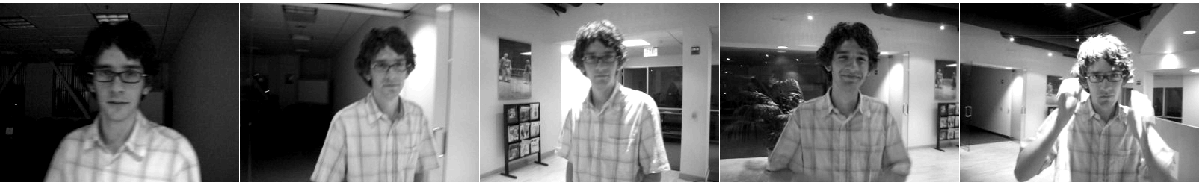
\includegraphics[height=0.45in]{thesis/seq_2_davidin300.png}\label{fig:trk_pca_1b}}
									\subfigure[Sylv.]{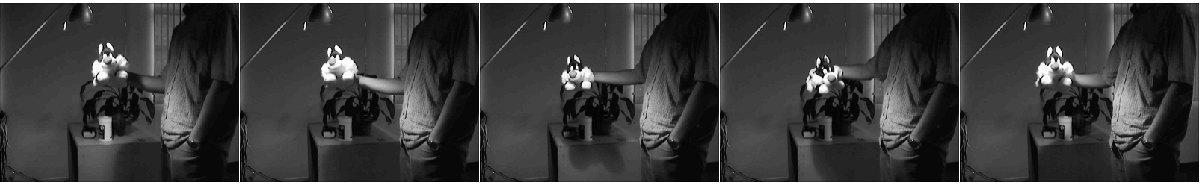
\includegraphics[height=0.45in]{thesis/seq_3_sylv.png}\label{fig:trk_pca_1c}}
									\subfigure[Fish.]{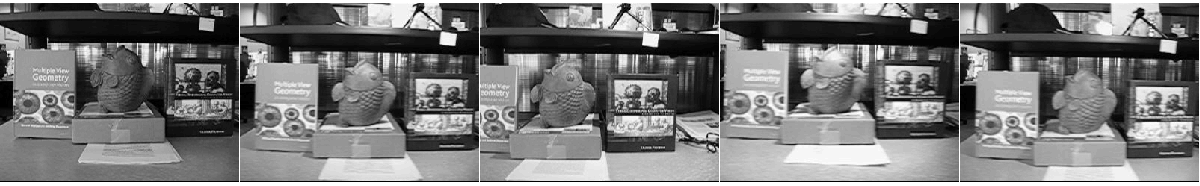
\includegraphics[height=0.45in]{thesis/seq_5_fish.png}\label{fig:trk_pca_1d}}
									\subfigure[Car4.]{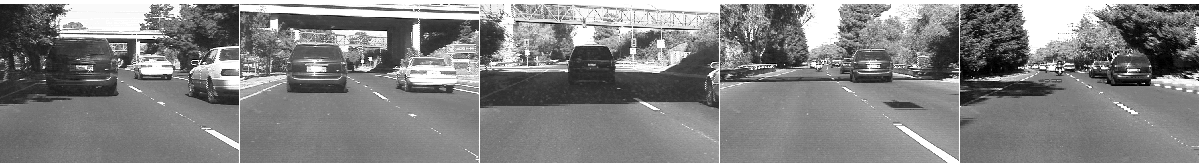
\includegraphics[height=0.45in]{thesis/seq_6_car4.png}\label{fig:trk_pca_1d}}
									\subfigure[Car11.]{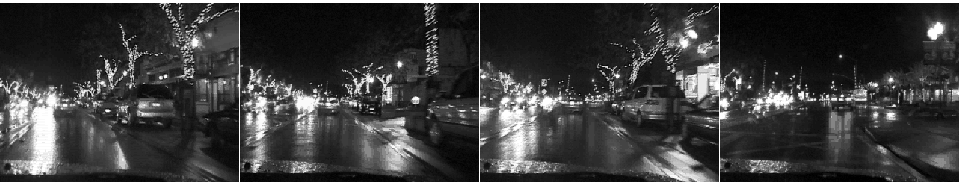
\includegraphics[height=0.45in]{thesis/seq_7_car11.png}\label{fig:trk_pca_1d}}
									\caption{Tracking sequences.}
									\label{fig:trk_pca}
									\end{figure}

%=========================
\section{Results}
%=========================
\begin{figure}[h!]
\centering
\begin{tabular}{|l|c|c|c|}
\hline
&\textbf{Q=8}&\textbf{Q=16}&\textbf{Q=32}\\\hline
\textbf{Dudek}&7.44&7.81&8.54\\\hline
\textbf{davidin300}&8.36&4.60&6.93\\\hline
\textbf{sylv}&4.34&5.47&5.72\\\hline
\textbf{fish}&9.75&2.17&7.98\\\hline
\textbf{car4}&4.79&4.60&5.52\\\hline
\textbf{car11}&2.21&2.13&2.39\\\hline
\end{tabular}

\subfigure[]{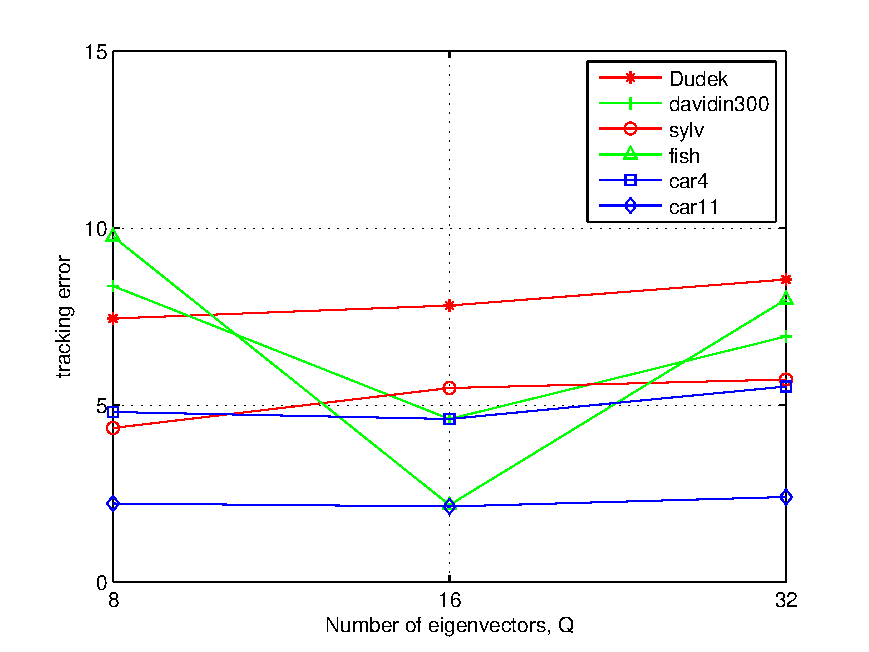
\includegraphics[width=0.45\textwidth]{temp/results_pca__trk_1a.pdf}\label{fig:trk_pca_1a}}
\subfigure[]{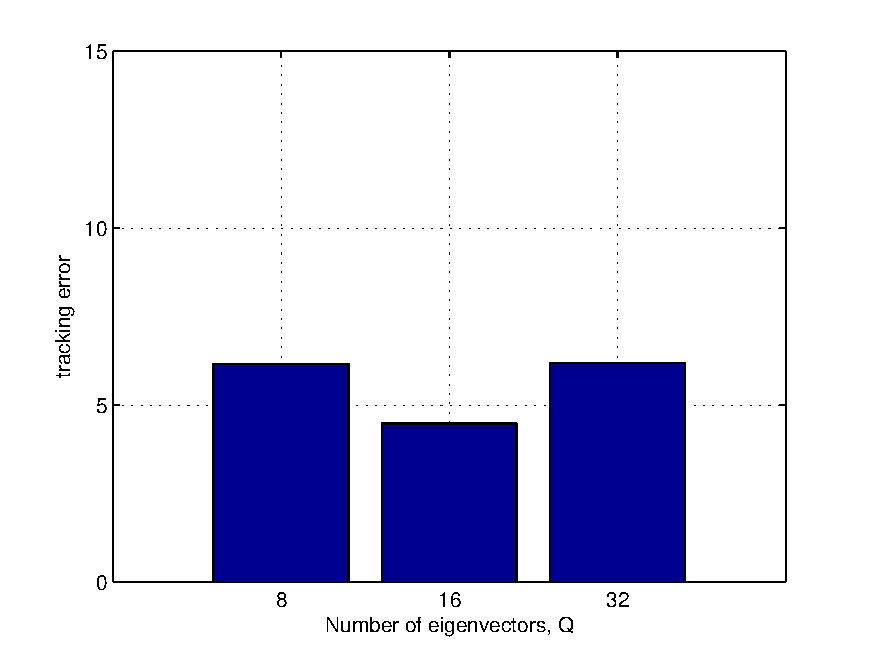
\includegraphics[width=0.45\textwidth]{temp/results_pca__trk_1b.pdf}\label{fig:trk_pca_1b}}
\subfigure[]{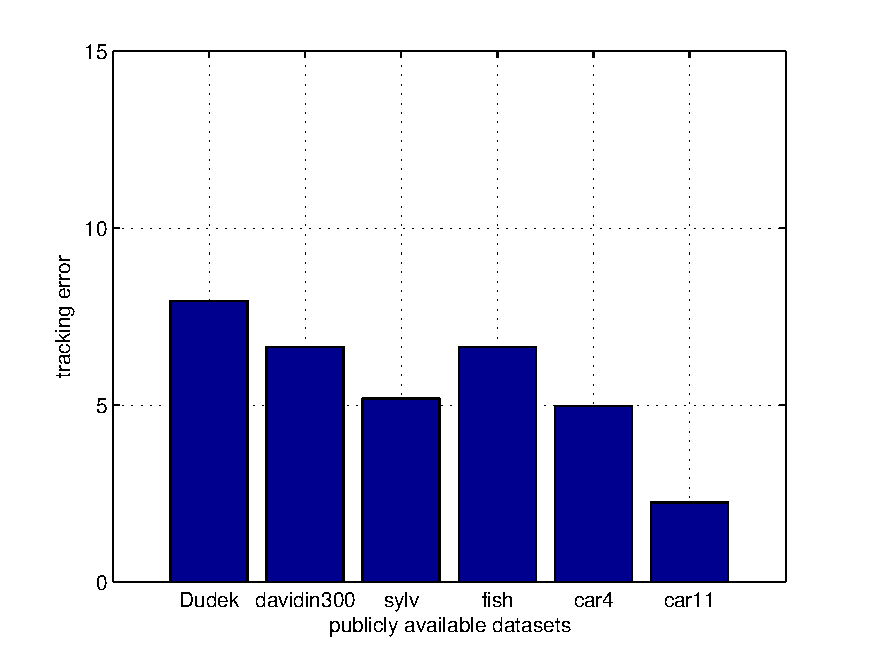
\includegraphics[width=0.45\textwidth]{temp/results_pca__trk_1c.pdf}\label{fig:trk_pca_1c}}
\subfigure[]{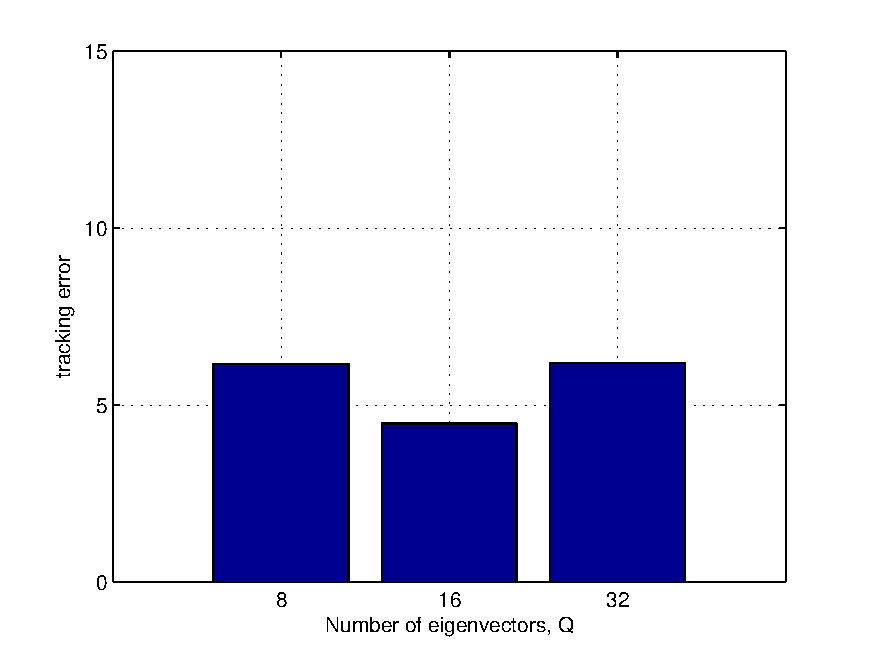
\includegraphics[width=0.45\textwidth]{temp/results_pca__trk_1d.pdf}\label{fig:trk_pca_1d}}
\caption{Tracking error for PCA based tracking for different number of eigenvectors $Q$ for 6 different publicly available datasets.}
\label{fig:trk_pca}
\end{figure}
Tracking error results are given in the table in Figure~\ref{fig:trk_pca}.  Each entry in this table represents tracking error temporally averaged over the frames of a dataset (most of the datasets have more than 500 images).  The entries in this table are visualized using 4 plots.  In Figures~\ref{fig:trk_pca_1a} and~\ref{fig:trk_pca_1b}, we plot the tracking error for different datasets and different values of $Q$ respectively.  The averages of these figures are plotted in Figures~\ref{fig:trk_pca_1c} and~\ref{fig:trk_pca_1d} respectively.  From these results, we make the following observations:


\begin{enumerate}
\item \underline{Variation in data}.
\begin{enumerate}
\item The Dudek and sylv sequences are characterized by some lighting variation but large pose variation.
\item The davidin300 and fish sequences are characterized by large lighting variation.
\item The car4 and car11 sequences have relatively less variation in lighting and pose.
\end{enumerate}
\item \underline{Continually increasing error}.  For Dudek and sylv, the error continues to increase from $Q=8$ to $Q=32$.
\item \underline{Sharply decreasing, then sharply increasing error}. For davidin300 and fish, the error decreases from $Q=8$ to $Q=16$, and then increases from $Q=16$ to $Q=32$.   The tracking error at $Q=16$ is significantly lower than for $Q=8$ and $Q=32$.
\item \underline{Mildly decreasing, then mildly increasing error}.  For car4 and car11, like for davidin300 and fish above, the error decreases from $Q=8$ to $Q=16$, and then increases from $Q=16$ to $Q=32$.  However, the drop and rise in error is not as steep.
\item \underline{Highest error}.  The average error for the Dudek sequence is highest.  This is because this sequence contains more variation than all other sequences including temporary occlusions, expression changes, structured noise, lighting changes and pose changes.  
\item \underline{Face tracking}.  For the Dudek sequence, we try to track a face.  In the context of faces, we first look at related areas,

\begin{enumerate}
\item \underline{Face reconstruction}.  It has been shown that 40 eigenfaces can be used to reconstruct a face with 3\% error~\cite{1987_JNL_Faces_Sirovich}.
\item \underline{Face recognition}.  Face recognition performance levels off at about 25 principal components, or 45 principal components if the first 3 principal components are dropped~\cite{1997_JNL_EigenVsFisherFaces_Bel}.
\item \underline{Accounting for lighting changes in face recognition}.  It has been shown that the first 3 principal components account for lighting changes in faces.  However, these components are unlikely to only account for lighting variation and removing them may result in loss of important information~\cite{1997_JNL_EigenVsFisherFaces_Bel}.
\end{enumerate}

Given these observations in related areas of facial processing, we do not remove any principal components.  However, unlike the face recognition case, our tracking performance does not keep increasing till 20 or more eigenvectors.  An important difference in tracking applications however is that face alignment is noisy.  It appears that in the Dudek and sylv (sylv is a cartoonish face) sequences which have large pose changes, the first few eigenvectors are able to capture the linear dependencies in the slightly shifted faces.  After that, the later eigenvectors explain the residual noise.  This can lead to decreased tracking performance since reconstructions using an eigenspace that partially explains noise will naturally be noisy.  Noisy reconstructions will get inaccurate DFFS (distance-from-feature-space) scores, which in turn will cause incorrect weighting for particle filter candidates in the tracking process.
\item \underline{Best Q is 16}.  Overall, on average, $Q=16$ produces the lowest tracking error.  On average, the tracking error decreases from $Q=8$ to $Q=16$, and then increases from $Q=16$ to $Q=32$.  It appears that the number of eigenvectors required to capture the linear correlation in these datasets is between 16 and 32, but closer to 16.   
The reason for the decrease in tracking error is that a certain number of eigenvectors are needed to capture the linear correlations in the data.  A subsequent increase in tracking error, as discussed earlier, appears to be related to the difficulty in correctly aligning the targets which causes later PCA eigenvectors to explain noise.
\end{enumerate}

%=========================
\section{Conclusions}
%=========================
In tracking scenarios, accurate alignment of targets is difficult.  In many cases, PCA with about 8 to 16 eigenvectors can capture the linear dependence between slightly shifted versions of the same target since slight shifts still preserve correlation.  However, as the number of eigenvectors increases further, the additional eigenvectors explain noise in the data.  This can lead to noisy reconstructions and subsequent noisy weighting for target candidates.  When the noisy target candidate that is best explained by the PCA subspace is then added to the training set to update the PCA subspace, the resulting subspace will be noisy which will further increase the chances of noisy reconstructions.  

In tracking scenarios, it is therefore recommended to use between 8 and 16 eigenvectors.


\normalsize
\bibliographystyle{ieee}
\bibliography{MyCitations}
\end{document}



%All images of a Lambertian surface\footnote{A Lambertian surface, or informally a matte surface, is a surface that has constant BRDF (bidirectional reflectance distribution function) $\rho(\theta_o, \phi_o, \theta_i, \phi_i)=\frac{L_o(x, \theta_o, \phi_o)}{L_i(x, \theta_i, \phi_i)\cos\theta_i d\omega}$, where the angles ($\theta_o, \phi_o$) define the outgoing light direction and angles ($\theta_i, \phi_i$) define the incoming light direction.  A surface illuminated by radiance $L_i(x, \theta_i, \phi_i)$ coming in from a differential region of solid angle $d\omega$ at angles $\theta_i, \phi_i$ receives irradiance $L_i(x, \theta_i, \phi_i)\cos\theta_i d\omega$.  Irradiance is measured in $\mathrm{W/m^2}$, while the solid angle $d\omega$ is measured in steridians, sr.  The unit of BRDF is therefore $\mathrm{sr^{-1}}$.} taken under different lighting conditions but from a fixed viewpoint lie on a 3D linear subspace of a high-dimensional image space \cite{1992_THE_GeoPhoto_Shashua}.  However, since this does not hold in practice due to shadowing, specularities, etc, modeling such changes with PCA can often lead to difficulties.  